% ----------------------------------------------------------------------
%                   LATEX TEMPLATE FOR PhD THESIS
% ----------------------------------------------------------------------

% based on Harish Bhanderi's PhD/MPhil template, then Uni Cambridge
% http://www-h.eng.cam.ac.uk/help/tpl/textprocessing/ThesisStyle/
% corrected and extended in 2007 by Jakob Suckale, then MPI-CBG PhD programme
% and made available through OpenWetWare.org - the free biology wiki


%: Style file for Latex
% Most style definitions are in the external file PhDthesisPSnPDF.
% In this template package, it can be found in ./Latex/Classes/
\documentclass[twoside,11pt]{Latex/Classes/PhDthesisPSnPDF}

%: Macro file for Latex
% Macros help you summarise frequently repeated Latex commands.
% Here, they are placed in an external file /Latex/Macros/MacroFile1.tex
% An macro that you may use frequently is the figuremacro (see introduction.tex)
% This file contains macros that can be called up from connected TeX files
% It helps to summarise repeated code, e.g. figure insertion (see below).

% insert a centered figure with caption and description
% parameters 1:filename, 2:title, 3:description and label
\newcommand{\figuremacro}[3]{
	\begin{figure}[htbp]
		\centering
		\includegraphics[width=1\textwidth]{#1}
		\caption[#2]{\textbf{#2} - #3}
		\label{#1}
	\end{figure}
}

% insert a centered figure with caption and description AND WIDTH
% parameters 1:filename, 2:title, 3:description and label, 4: textwidth
% textwidth 1 means as text, 0.5 means half the width of the text
\newcommand{\figuremacroW}[4]{
	\begin{figure}[htbp]
		\centering
		\includegraphics[width=#4\textwidth]{#1}
		\caption[#2]{\textbf{#2} - #3}
		\label{#1}
	\end{figure}
}

% inserts a figure with wrapped around text; only suitable for NARROW figs
% o is for outside on a double paged document; others: l, r, i(inside)
% text and figure will each be half of the document width
% note: long captions often crash with adjacent content; take care
% in general: above 2 macro produce more reliable layout
\newcommand{\figuremacroN}[3]{
	\begin{wrapfigure}{o}{0.5\textwidth}
		\centering
		\includegraphics[width=0.48\textwidth]{#1}
		\caption[#2]{{\small\textbf{#2} - #3}}
		\label{#1}
	\end{wrapfigure}
}

% predefined commands by Harish
\newcommand{\PdfPsText}[2]{
  \ifpdf
     #1
  \else
     #2
  \fi
}

\newcommand{\IncludeGraphicsH}[3]{
  \PdfPsText{\includegraphics[height=#2]{#1}}{\includegraphics[bb = #3, height=#2]{#1}}
}

\newcommand{\IncludeGraphicsW}[3]{
  \PdfPsText{\includegraphics[width=#2]{#1}}{\includegraphics[bb = #3, width=#2]{#1}}
}

\newcommand{\InsertFig}[3]{
  \begin{figure}[!htbp]
    \begin{center}
      \leavevmode
      #1
      \caption{#2}
      \label{#3}
    \end{center}
  \end{figure}
}

\newcommand{\tab}[1]{\hspace{.2\textwidth}\rlap{#1}}

%%% Local Variables: 
%%% mode: latex
%%% TeX-master: "~/Documents/LaTeX/CUEDThesisPSnPDF/thesis"
%%% End: 

       
% turn of those nasty overfull and underfull hboxes
\hbadness=10000
\hfuzz=50pt

%: --------------------------------------------------------------
%:                  NEW COMMANDS: definitions
% --------------------------------------------------------------

\newcommand{\HRule}{\rule{\linewidth}{0.5mm}}

%: --------------------------------------------------------------
%:                  FRONT MATTER: dedications, abstract,..
% --------------------------------------------------------------

\begin{document}

% sets line spacing
\renewcommand\baselinestretch{1.2}
\baselineskip=18pt plus1pt

%: ----------------------- UT cover page ------------------------

\begin{titlepage}

\begin{center}



\textsc{UNIVERSITY OF TARTU}\\

\textsc{FACULTY OF MATHEMATICS AND COMPUTER SCIENCE}\\

\texttt{Institute of Computer Science}\\

\vspace{6 cm}


% Title
%\HRule \\[0.4cm]
\textsc{ \large Jaan Tohver}\\[0.5cm]
{ \Huge \bfseries Gesture Ads for Mobile Applications}\\[0.5cm]
{\large Bachelor Thesis (6 EAP)}\\[3cm]


%\HRule \\[1.5cm]

% Author and supervisor
%\begin{minipage}{0.4\textwidth}
%\begin{flushleft} \large
%\emph{Author:}\\
%John \textsc{Smith}
%\end{flushleft}
%\end{minipage}
\begin{minipage}{0.8\textwidth}
\begin{flushright} \large
\emph{Supervisor: Huber Flores, Msc}  \\	  %degree (e.g. Phd, Msc, etc.)
 %\textsc{Brown}
\end{flushright}
\end{minipage}

\textbf{}\\[1.0cm]

\textbf{Author:.................................... "....." May   2015}\\[0.5cm]

\textbf{Supervisor:............................... "....." May   2015}\\[0.5cm]

\textbf{Professor:................................. "....." May   201X}\\[0.5cm]        

\vfill

% Bottom of the page
{\large TARTU, 2015}

\end{center}

\end{titlepage}


%: ----------------------- abstract ------------------------


% Thesis Abstract -----------------------------------------------------

\begin{abstracts}        %this creates the heading for the abstract page

Mobile advertising is an inseparable part in today's mobile application development. In many cases advertising enables the developer to offer their application to users for free. However, more often than not, in-application advertisements prove to be distracting to the user and, in extreme cases, even degrade the user experience to a point where the user decides to stop using the application. In any case, the user most often tends to just ignore the advertisements, which makes the advertising model ineffective and compromises the reputation of the application without significant gain for any party.

The goal of this project is to develop a library that application developers can use, which would integrate advertisements more seamlessly into the flow of the application. It would allow the application to receive all the necessary data via a push notification from the server and then display a very minimalist form of it to the user, without taking up too much of the very limited screen space of the device. The application will then hopefully still retain usability for any time-critical activities.

The user can focus his/her attention on the advertisement when the time is most suitable (e.g. they have finished reading a paragraph). The user can then use a spread motion to view more a detailed description of the advertisement or flick it either left to show disinterest or right to show interest – a motion many mobile users are already conceptually familiar with. Data will then be sent back to the server to be processed and, based on the processed data, the future advertisements can be more suited to the user's interests. Showing interest in the advertisement will also store it for future viewing, should the user wish to do so. If the user chooses to ignore the advertisement, it will remain on the screen for a period of time and then disappear.

Another use case would be to incorporate the user's current location to the process. This would allow the user to receive advertisements not only relevant in terms of their interests, but also in terms of their current location.

By the end, the library will hopefully serve three purposes:

\begin{itemize}
  \item It will make the application more enjoyable for the user, by offering less intrusive methods of advertising and advertisements more relevant to the individual user.
  \item It will make incorporating mobile advertisements easier for the developer and give the developer more freedom to focus on user experience, without having to worry about advertising mechanics.
  \item It will allow the advertiser to offer content relevant to the user, thereby increasing the user's perception of the product as well as the likelihood of the user choosing to learn more about the offer.
\end{itemize}

\end{abstracts}

% ---------------------------------------------------------------------- 

% The original template provides and abstractseparate environment, if your institution requires them to be separate. I think it's easier to print the abstract from the complete thesis by restricting printing to the relevant page.
% \begin{abstractseparate}
%   
% Thesis Abstract -----------------------------------------------------

\begin{abstracts}        %this creates the heading for the abstract page

Mobile advertising is an inseparable part in today's mobile application development. In many cases advertising enables the developer to offer their application to users for free. However, more often than not, in-application advertisements prove to be distracting to the user and, in extreme cases, even degrade the user experience to a point where the user decides to stop using the application. In any case, the user most often tends to just ignore the advertisements, which makes the advertising model ineffective and compromises the reputation of the application without significant gain for any party.

The goal of this project is to develop a library that application developers can use, which would integrate advertisements more seamlessly into the flow of the application. It would allow the application to receive all the necessary data via a push notification from the server and then display a very minimalist form of it to the user, without taking up too much of the very limited screen space of the device. The application will then hopefully still retain usability for any time-critical activities.

The user can focus his/her attention on the advertisement when the time is most suitable (e.g. they have finished reading a paragraph). The user can then use a spread motion to view more a detailed description of the advertisement or flick it either left to show disinterest or right to show interest – a motion many mobile users are already conceptually familiar with. Data will then be sent back to the server to be processed and, based on the processed data, the future advertisements can be more suited to the user's interests. Showing interest in the advertisement will also store it for future viewing, should the user wish to do so. If the user chooses to ignore the advertisement, it will remain on the screen for a period of time and then disappear.

Another use case would be to incorporate the user's current location to the process. This would allow the user to receive advertisements not only relevant in terms of their interests, but also in terms of their current location.

By the end, the library will hopefully serve three purposes:

\begin{itemize}
  \item It will make the application more enjoyable for the user, by offering less intrusive methods of advertising and advertisements more relevant to the individual user.
  \item It will make incorporating mobile advertisements easier for the developer and give the developer more freedom to focus on user experience, without having to worry about advertising mechanics.
  \item It will allow the advertiser to offer content relevant to the user, thereby increasing the user's perception of the product as well as the likelihood of the user choosing to learn more about the offer.
\end{itemize}

\end{abstracts}

% ---------------------------------------------------------------------- 
% \end{abstractseparate}

%: ----------------------- contents ------------------------

\setcounter{secnumdepth}{3}		% organisational level that receives a numbers
\setcounter{tocdepth}{3}    		% print table of contents for level 3
\tableofcontents            				% print the table of contents
% levels are: 0 - chapter, 1 - section, 2 - subsection, 3 - subsection

%: ----------------------- list of figures/tables ------------------------

%\listoffigures	% print list of figures

%\listoftables  % print list of tables

%: ----------------------- glossary ------------------------

% Tie in external source file for definitions: /0_frontmatter/glossary.tex
% Glossary entries can also be defined in the main text. See glossary.tex
%% this file is called up by thesis.tex
% content in this file will be fed into the main document

% Glossary entries are defined with the command \nomenclature{1}{2}
% 1 = Entry name, e.g. abbreviation; 2 = Explanation
% You can place all explanations in this separate file or declare them in the middle of the text. Either way they will be collected in the glossary.

% required to print nomenclature name to page header
\markboth{\MakeUppercase{\nomname}}{\MakeUppercase{\nomname}}


% ----------------------- contents from here ------------------------

% chemicals
\nomenclature{DAPI}{4',6-diamidino-2-phenylindole; a fluorescent stain that binds strongly to DNA and serves to marks the nucleus in fluorescence microscopy} 
\nomenclature{DEPC}{diethyl-pyro-carbonate; used to remove RNA-degrading enzymes (RNAases) from water and laboratory utensils}
\nomenclature{DMSO}{dimethyl sulfoxide; organic solvent, readily passes through skin, cryoprotectant in cell culture}
\nomenclature{EDTA}{Ethylene-diamine-tetraacetic acid; a chelating (two-pronged) molecule used to sequester most divalent (or trivalent) metal ions, such as calcium (Ca$^{2+}$) and magnesium (Mg$^{2+}$), copper (Cu$^{2+}$), or iron (Fe$^{2+}$ / Fe$^{3+}$)}



 

%\begin{multicols}{2} % \begin{multicols}{#columns}[header text][space]
%\begin{footnotesize} % scriptsize(7) < footnotesize(8) < small (9) < normal (10)

%\printnomenclature[1.5cm] % [] = distance between entry and description
%\label{nom} % target name for links to glossary

%\end{footnotesize}
%\end{multicols}

%%%%%%%%%%%%%%%%%%%%%%%%%%%%%%%%%%%INCLUDE LATEX SUBDOCUMENTS%%%%%%%%%%%%%%%%%%%%%%%%%%%%%%%%%%%%%%%%%%%%

%: --------------------------------------------------------------
%:                  MAIN DOCUMENT SECTION
% --------------------------------------------------------------

% the main text starts here with the introduction, 1st chapter,...
\mainmatter

\renewcommand{\chaptername}{} % uncomment to print only "1" not "Chapter 1"


%: ----------------------- subdocuments ------------------------

% Parts of the thesis are included below. Rename the files as required.
% But take care that the paths match. You can also change the order of appearance by moving the include commands.


% this file is called up by thesis.tex
% content in this file will be fed into the main document

%: ----------------------- introduction file header -----------------------
\chapter{Introduction}

% the code below specifies where the figures are stored
\ifpdf
    \graphicspath{{1_introduction/figures/PNG/}{1_introduction/figures/PDF/}{1_introduction/figures/}}
\else
    \graphicspath{{1_introduction/figures/EPS/}{1_introduction/figures/}}
\fi

% ----------------------------------------------------------------------
%: ----------------------- introduction content -----------------------
% ----------------------------------------------------------------------



%: ----------------------- HELP: latex document organisation
% the commands below help you to subdivide and organise your thesis
%    \chapter{}       = level 1, top level
%    \section{}       = level 2
%    \subsection{}    = level 3
%    \subsubsection{} = level 4
% note that everything after the percentage sign is hidden from output

Mobile advertising is an inseparable part in today's mobile application development. In many cases advertising enables the developer to offer their application to users for free. The most common way advertisements are displayed to the user is taking up a big part, if not all, of the device's screen real estate giving the developer little control of the content of the advertisements; often tricking users into clicking the link within the advertisement instead of closing it.

\section{Motivation}
More often than not, in-application advertisements prove to be distracting to the user and, in extreme cases, even degrade the user experience to a point where the user decides to stop using the application.  In addition, usually the user tends to just ignore the advertisements. This makes the advertising model ineffective and compromises the reputation of the application, as well as the developer, without significant gain for any party.

Advertisements influence people's attitude towards advertising by a great deal. When advertisements employ techniques that irritate or bother the user, then the user is likely to perceive them as an unwanted influence.\cite{chowdhury2010consumer} A less intrusive and more intuitive, user feedback based method of displaying advertisements would improve the user experience of the application with the added benefit of users being more likely to see the content of the advertisement.

\section{Contributions}
### (polish the sentence) The goal of this thesis is to describe current advertisment models for mobile apps and explore new mechanisms to deliver ads, which are not as intrusive as current solutions.

As a result, we design and implement a new mechanisms namely \textit{Gesture ads}. Our mechanism....(here you describe the mechanism)

To distribute our mechanisms we create a Java library for Android \cite{android:platform} ...... platform that application developers can use, which would integrate advertisements more seamlessly into the flow of the application. It would allow the application to receive all the necessary data via a push notification from the server and then display a very minimalist form of it to the user, without taking up too much of the very limited screen space of the device. The application should still retain usability for any time-critical activities with the advertisement being movable if necessary.

The user can focus their attention on the advertisement when the time is most suitable. They can then use a spread gesture to view a more detailed description of the advertisement or flick it either left to show disinterest or right to show interest. Data will then be sent back to the server to be processed and stored. Showing interest in the advertisement will also store it for future viewing, should the user wish to do so. If the user chooses to ignore the advertisement, it will remain on the screen for a period of time and then disappear.

The server application can then take into account, among other things, the user's preferred topics and location to send advertisements more relevant to the user.

By the end, the library will serve three purposes:
\begin{itemize}
  \item To make the application more enjoyable for the user, by offering less intrusive methods of advertising and advertisements more relevant to the individual user.
  \item (polish this one) To ease the integration of mobile advertisements easier into the mobile apps and give the developer more freedom to focus on user experience, without having to worry about advertising mechanics.
  \item (rewrite starting with "To ...") It will allow the advertiser to offer content relevant to the user, thereby increasing the user's perception of the product as well as the likelihood of the user choosing to learn more about the offer.
\end{itemize}

\section{Outline}
\noindent \textbf{Chapter 2}: describes the most popular mobile advertising frameworks used today and discusses the pros and cons of each. It also takes a closer look at some of the more unorthodox advertising frameworks that do not follow the most common patterns of mobile advertising and take user experience regarding mobile advertisements to the next level.

\noindent \textbf{Chapter 3}: describes in detail the development process and the final structure of the font-end library as well as the server application used to test the library.

\noindent \textbf{Chapter 4}: takes a closer look at user feedback regarding the developed library as well as mobile advertisements in general. Brief analysis.
		% background information
% this file is called up by thesis.tex
% content in this file will be fed into the main document

%: ----------------------- name of chapter  -------------------------
\chapter{Problem Statement} % top level followed by section, subsection


%transition between chapters, usually no more than two parragraphs
Transition - Since the establishment of SyncML by the Open Handset Alliance (OHA); the synchronization of data is the adopted approach for supplying cloud resources to the handset... 



%: ----------------------- paths to graphics ------------------------

% change according to folder and file names
\ifpdf
    \graphicspath{{X/figures/PNG/}{X/figures/PDF/}{X/figures/}}
\else
    \graphicspath{{X/figures/EPS/}{X/figures/}}
\fi

%: ----------------------- Mobile Cloud Middleware ------------------------

\section{Research Question}
Engineering theses tend to refer to a problem to be solved where other disciplines talk in terms of a question to be answered. In either case, this section has three main parts: 
1. a concise statement of the question that your thesis tackles 
2. justification, by direct reference to section 3, that your question is previously unanswered
3. discussion of why it is worthwhile to answer this question. 




%Summary of each chapter is MANDATORY
\section{Summary}
%example
To counter the problems with the interoperability across multiple clouds, to perform data-intensive processing invocation from the handset and to introduce the platform independence feature for the mobile cloud applications, the following thesis discusses a Mobile Cloud Middleware (MCM). The middleware provides a unique interface for mobile connection and multiple internal interfaces and adapters, which manage the connection and communication between different clouds. The MCM capabilities for managing the resource intensive tasks can easily be envisioned in several scenarios which are discussed in further sections as case of study. 





% ---------------------------------------------------------------------------
%: ----------------------- end of thesis sub-document ------------------------
% ---------------------------------------------------------------------------

					% problem statement
% this file is called up by thesis.tex
% content in this file will be fed into the main document

\chapter{Background} % top level followed by section, subsection

%transition between chapters, usually no more than two paragraphs

% ----------------------- State of the art ------------------------

\section{Classical Advertising Frameworks}

According to a 2012 article by Matt Marshall, the most reliable companies in mobile advertising, that directly offer a monetization service for the mobile platform, are AdMob, Millennial Media, iAd, Flurry, InMobi, Chartboost, MoPub and Amobee. \cite{mmarshall-top10} Following is a short overview of these eight platforms.

AdMob was founded in 2006 and acquired by Google in 2010. \cite{crunchbase-admob} According to research firm eMarketer Google is, by a large margin, the leader of the global digital ad market. \cite{emarketer-google} At the time of Google acquiring AdMob it was one of the market leaders in mobile advertising. \cite{google-admob} In 2011 it was merged with their existing AdSense platform, which is a solution for web advertising. \cite{admob-adsense} AdSense has software development kits (SDKs) for Android, iOS and Windows Phone \cite{admob-sdk}  and supports displaying in-app advertisements as a rectangle, a banner \cite{admob-banner} or a full screen interstitial.\cite{admob-interstitial}

Millennial Media was founded in 2006. \cite{crunchbase-millenial} Apart from Google, it is the only other mobile advertising company in the eMarketer list of top ten global digital advertising companies. \cite{emarketer-google} They offer an end-to-end technology stack with SDKs for Android, iOS, BlackBerry and Symbian. \cite{millenial-sdk} Ads can be displayed as a rectangle, banner or interstitial. \cite{millenial-android}

Like Google, in 2010 Apple acquired a mobile advertising company -- Quattro, founded in 2006. \cite{crunchbase-quattro} It was then rebranded as iAd \cite{forbes-iad}, which has not seen much success to date and, according to an article posted on Forbes, only accounts for 2.5\% of mobile advertising revenues in the United States. \cite{forbes-iad2} iAd only supports iOS and the advertisements are native, meaning that the developer can define the bounds of the advertisement with x and y coordinates, width and height. \cite{iad-tutorial}

Flurry was founded in 2005 and acquired by Yahoo in July of 2014. \cite{crunchbase-flurry} The main selling point of Flurry is its analytics tool with the largest data-set on application usage. \cite{maps-yankeegroup} Flurry supports Android and iOS and the advertisements can be displayed as either a banner or full screen.

InMobi was founded in 2007. \cite{crunchbase-inmobi} They claim to be the first advertising platform with 1 billion unique users. \cite{inmobi} InMobi supports Android, iOS and Windows Phone \cite{inmobi-monetize} and the advertisements can be displayed as a banner, full screen or native. \cite{inmobi-sdk}

Chartboost was founded in 2011. \cite{crunchbase-chartboost} It is a mobile games-only advertisement network and focuses on cross promotion of mobile games, meaning that most of the advertisements are about downloading other games. According to their own words it only takes ten lines of code to integrate Chartboost into an application. \cite{chartboost} It supports Android and iOS and the advertisements can only be displayed full screen.\cite{hongikiat-monetize}

MoPub was founded in 2010 and acquired by Twitter in 2013. \cite{crunchbase-mopub} Their main selling point is a large real-time bidding exchange for in-application advertisements. This means that there is no sales person between the advertiser and the developer. Advertisers bid directly for the opportunity to have their advertisements displayed in an application and developers have  control and transparency over the ads that are delivered into the application. \cite{mopub-marketplace} Supported platforms are Android and iOS. \cite{mopub-resources} Supported formats are banner, full screen and native.

Amobee was founded in 2005 and acquired by SingTel in 2012. \cite{crunchbase-amobee} They have SDKs for Android, iOS, Windows Phone and BlackBerry. Possible formats are banners and full screen video.

Common for all these advertising platforms is the fact that none of them offer a format where the user can interact with the advertisement apart from tapping on it and, in case of full screen ads, close it. That is not to say that attempts haven’t been made to make advertisements interactable and/or more fun for the user.

\section{Dynamic Advertising Frameworks}

In 2009 apparel maker Dockers San Francisco launched an advertisement for iPhone, which used the phone’s accelerometer to respond to the user shaking their phone, which would then make a dancer, appearing on the screen, perform his moves. Dockers themselves believe that it was the first motion sensitive mobile advertisement. It was featured in iPhone games “iBasketball”, “iGolf” and “iBowl”.\cite{dockers}

Since then many advertisers have taken to offering advertisements using the phone’s sensors to make them more interesting to the user. Most notable perhaps is Adtile, which uses advertisements built with standard web technologies, using a JavaScript Motion Framework which gives access, among other things, to the device’s sensors and GPS, to make their advertisements fully interactable. Adtile supports Android and iOS devices. \cite{adtile}

But sometimes, even though the advertisements are interesting, the user just wants to continue using the application they were using with minimal interruption by displayed advertisements. An article titled “Can In-App Ads be Less Annoying for Smartphone Users?” by Huber Flores, Pan Hui and Yong Li proposes a framework that would split advertisements into smaller pieces and embed them into 2D objects, such as obstacles or collectable items, in a level of a mobile game. The advertisement would then be displayed to the user over a period of time, without taking away any extra screen real estate. \cite{gesture-ads}

\section{Related Works}

\section{Summary}

As it stands, there are no well known, easy to implement libraries to display responsive advertisements in classical mobile applications. Next section describes the proposed solution in detail.

% ---------------------------------------------------------------------------
% -----------------------end of thesis sub-document----------------
% --------------------------------------------------------------------------- 	        				% state of the art
\chapter{Implementation}


(An overview figure of the system is missing)


To demonstrate the feasibility of the proposed approach, a Java library for Android is developed. Also, a server application is developed for testing the library.

\section{Application library}

The library is a lightweight API that consists mainly of two parts: communication with the server,  and the ad view. The components of the server communication part are as follows:

\textit{AdContentLoader} is the only class that the application developer should ever have the need to call. An instance of it is initialised in an activity's \textit{onCreate} method. It then adds the ad view to the activity's content view, registers a broadcast receiver to receive messages from the server and registers the device to Google Cloud Messaging service (GCM).\cite{notifications:gcm} The application developer should also call \textit{onPause} and \textit{destroy} methods in the activity's corresponding methods, the first of which unregisters from GCM and the second unregisters the broadcast receiver and disposes the GCM connection. The developer can also set the position of the appearing advertisement through this class.

\textit{GCMIntentService} is a subclass of \textit{GCMBaseIntentService} and responsible for handling communication from GCM. \textit{onRegistered} method is called when the device is registered to GCM and makes a call to register to our back-end with the registration id from GCM. \textit{onUnregistered} unregisters the device from our back-end once it was unregistered from GCM. \textit{onMessage} receives and decodes the information about an advertisement that was sent from the server. There are also methods for receiving and handling server-side errors.

The \textit{ServerUtilities} class is an abstraction layer for communicating with our server. It has methods for registering and unregistering the device that are called in \textit{GCMIntentService} as discussed previously.

Finally, \textit{FileDownloader} is responsible for downloading the image files for an advertisement once \textit{GCMIntentService} receives and decodes them.

The user interface portion of the library is in a single class: \textit{DynamicAdView}. It is responsible for the displaying the advertisement as well as handling the user's gestures. The view is invisible until \textit{FileDownloader} notifies \textit{AdContentLoader} that images for an advertisement have been downloaded. \textit{AdContentLoader} then prompts the view to update itself with the new images. The view is then capable of handling pan, zoom and flick gestures. When the user moves the view out of the screen's bounds it remains invisible until another update notification.

\section{Back-end distributor}

On the server-side there is a Java server application that handles the client's requests. The main components of the application are as follows:

\textit{Datastore} is a simple implementation of a data store using standard Java collections. It is not persistent throughout redeploys, but its only purpose is to store the ids of registered devices.

\textit{RegisterServlet} takes as a parameter the registration id from GCM and adds it to \textit{Datastore}'s id list. Likewise, \textit{UnregisterServlet} takes as a parameter the registration id from that a device is registered with and removes it from \textit{Datastore}'s id list.

\textit{HomeServlet} is the only servlet with a graphical user interface. It has a label displaying the amount of registered devices as well as buttons to send pre-determined advertisements to the registered devices.

\textit{SendAllMessagesServlet} is responsible for sending a push notification to each of the registered devices once a button in \textit{HomeServlet} is pressed. It takes as a parameter the id of an advertisement and based on that builds a GCM message which it then sends to the devices, tracking whether sending the message was successful or not and then returning to \textit{HomeServlet}

\section{Summary}

As can be seen, the implementation is really minimalistic. However the library can be added to any Android application written in Java and the simple back-end application can be used to demonstrate the proposed method of displaying advertisements to a mobile user.

The next paragraph discusses the method used for gathering user feedback and analyses the results to support the hypothesis that the proposed method improves user experience over classical advertising methods.						% how the solution solved the problem - your solution
\chapter{Case Studies}

An application's user is generally not happy about seeing advertisements in the application. They degrade the overall experience and distract from the contents of the application itself. However, for some developers, advertisements are the only way to monetize their application.

In this chapter we try to determine how the proposed advertising methods compares to the more traditional ones in terms of user experience.

\section{Validation}

\textbf{Setup and Methodology:} To validate the hypothesis, the proposed solution is compared to traditional advertisement frameworks in terms of intrusiveness and effectiveness. A use case based on a Wikipedia app \footnote{https://github.com/wikimedia/WikipediaMobile} is developed, which implements the advertising library. This application is selected because the mechanism targets applications that present content to the user such as news, feeds, text, etc.

Initially, we integrate  traditional advertisement mechanisms into the selected application as shown in Figure \ref{fig:ads1}.

Next, we use the same Wikipedia application, but this time with our proposed solution implemented as seen in Figures \ref{fig:ads2} and \ref{fig:ads3}.


\begin{figure}
\begin{center}
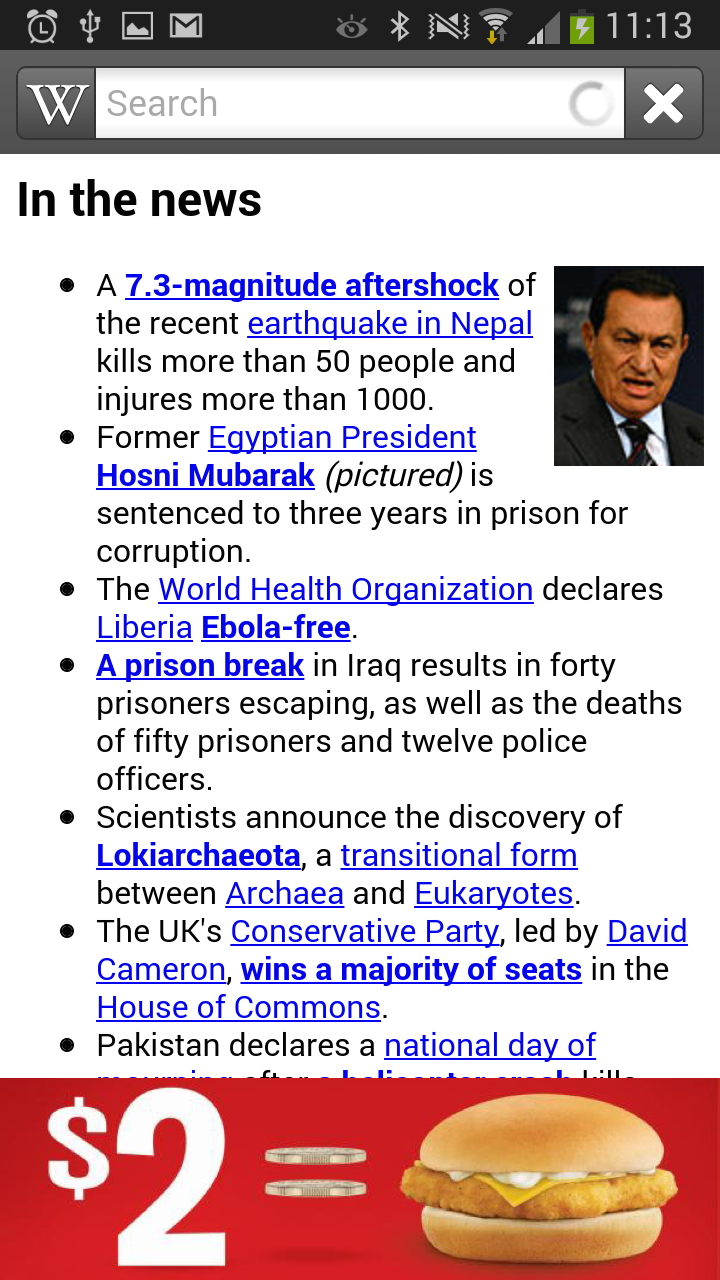
\includegraphics[scale=0.25]{Images/classicalad_banner.png}
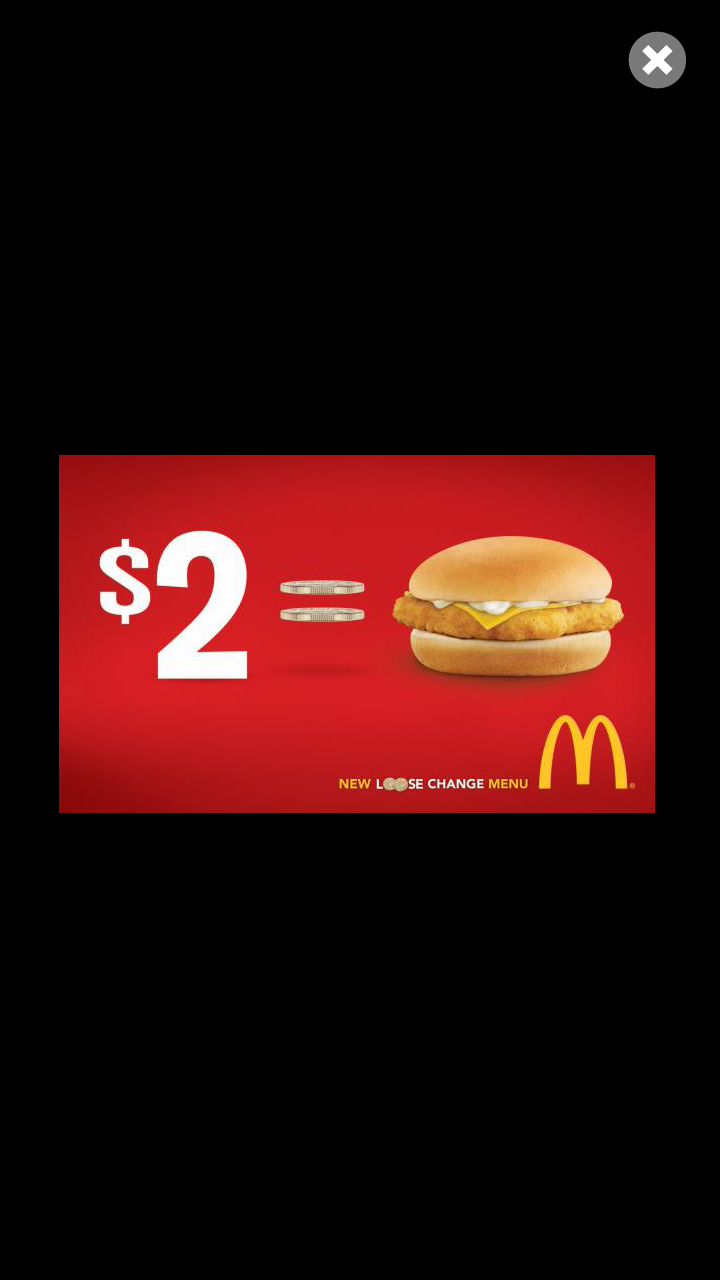
\includegraphics[scale=0.25]{Images/classicalad_fullscreen.png}
\caption{Examples of the application a banner or full screen advertisement}
\label{fig:ads1}
\end{center}
\end{figure}

Figure 5.2 shows what the application might look like right after a \textit{Gestrure Ad} appears and how it might look like after the user moves it to finish their reading.

\begin{figure}
\begin{center}
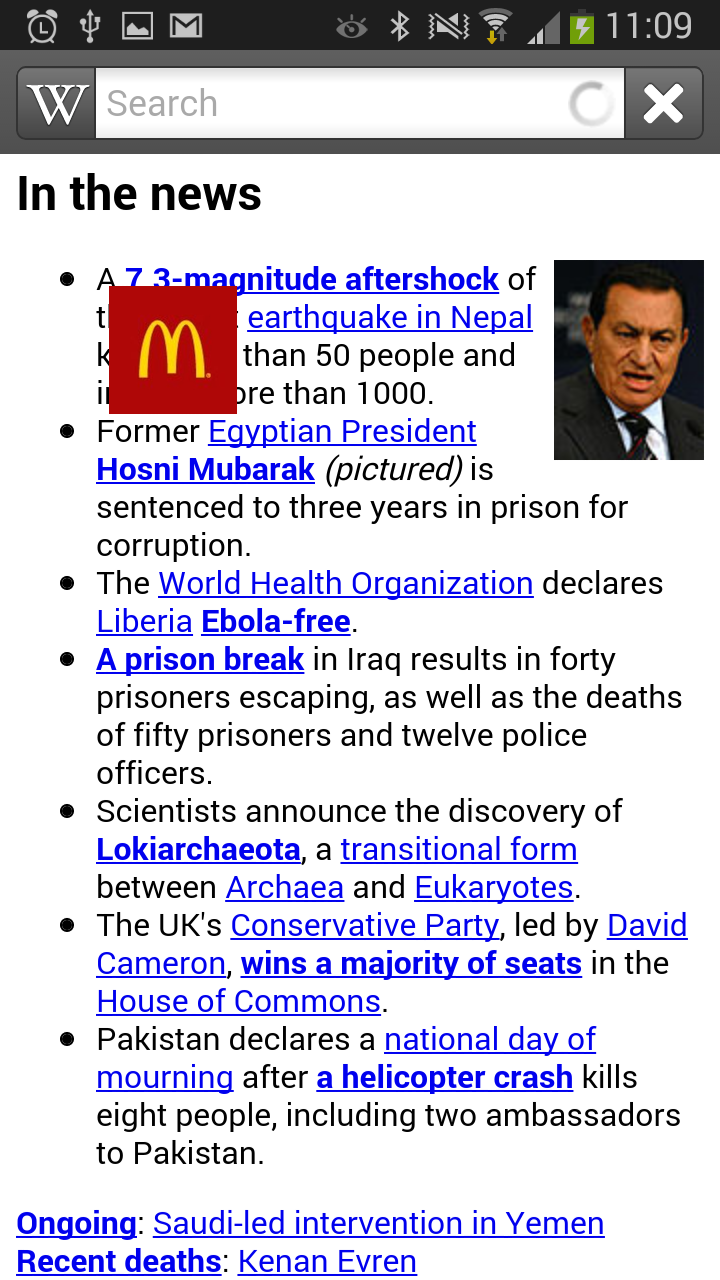
\includegraphics[scale=0.25]{Images/gesturead_small1.png}
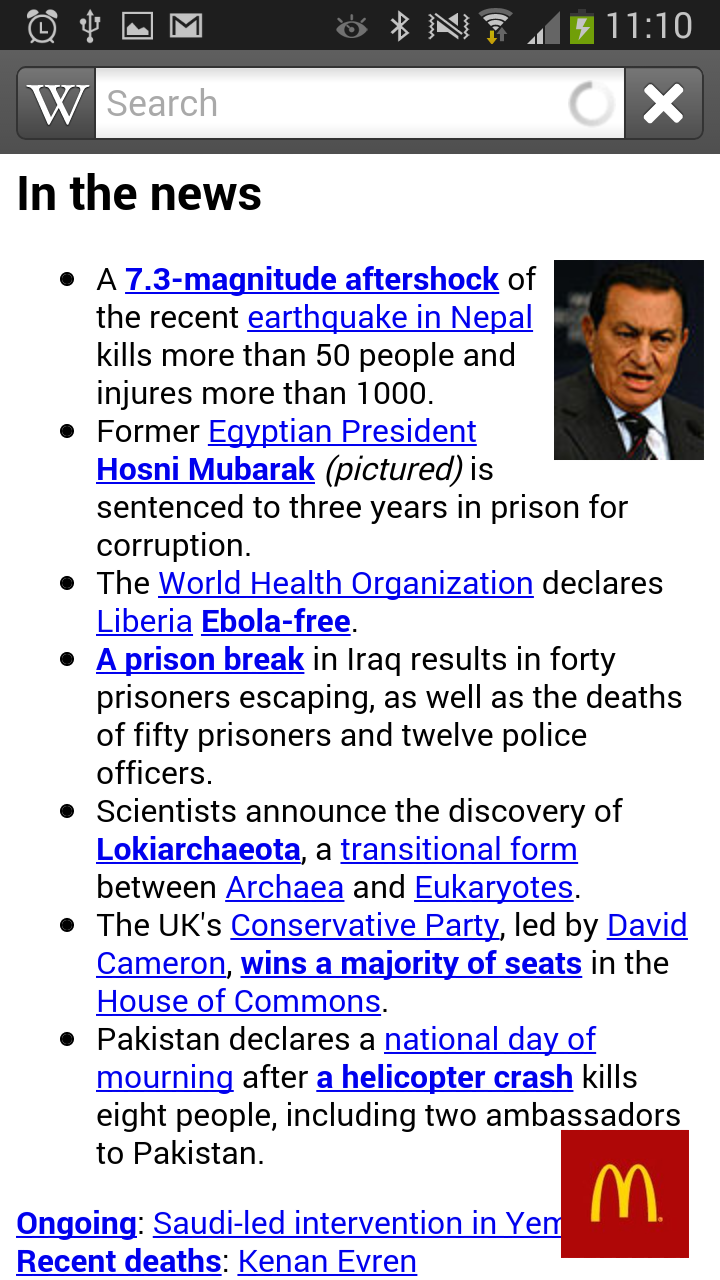
\includegraphics[scale=0.25]{Images/gesturead_small2.png}
\caption{Examples of the application with a \textit{Gestrure Ad} in minimised form displayed}
\label{fig:ads2}
\end{center}
\end{figure}

Figure 5.3 shows what the application might look like after the user zooms in on the advertisement and how it might look like after the user has started dragging it left to indicate disinterest in it.

\begin{figure}
\begin{center}
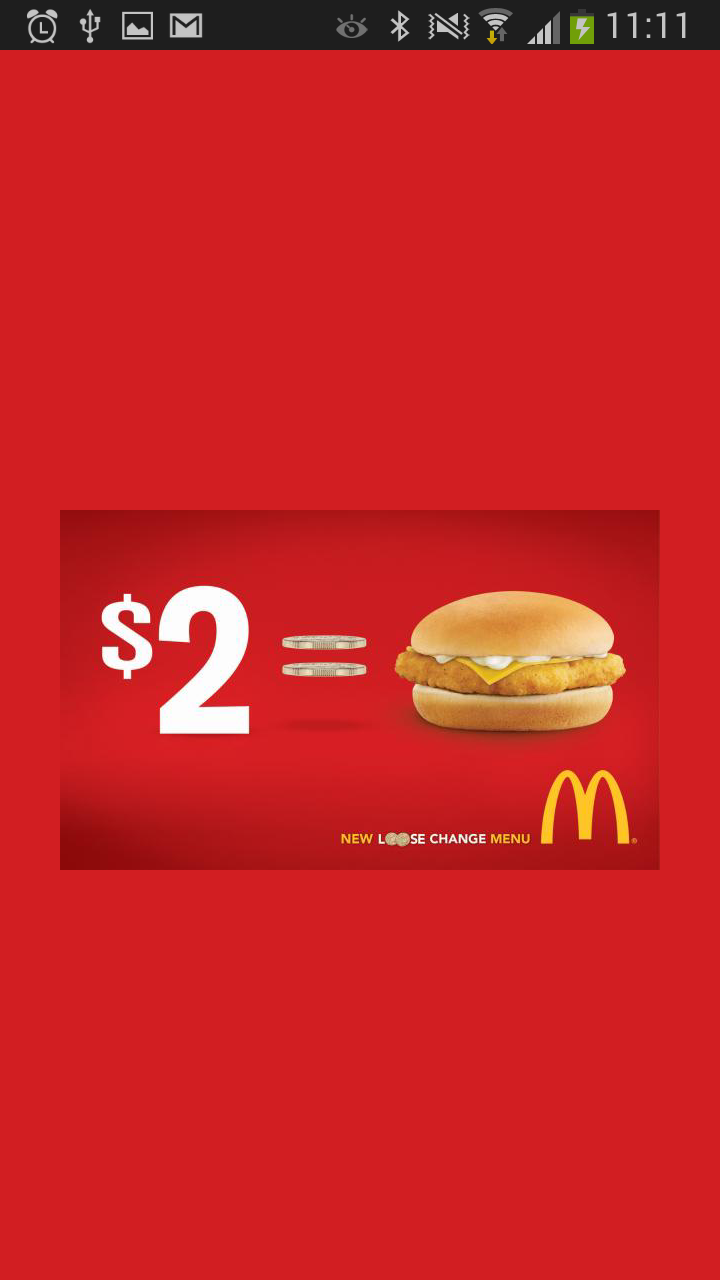
\includegraphics[scale=0.25]{Images/gesturead_big1.png}
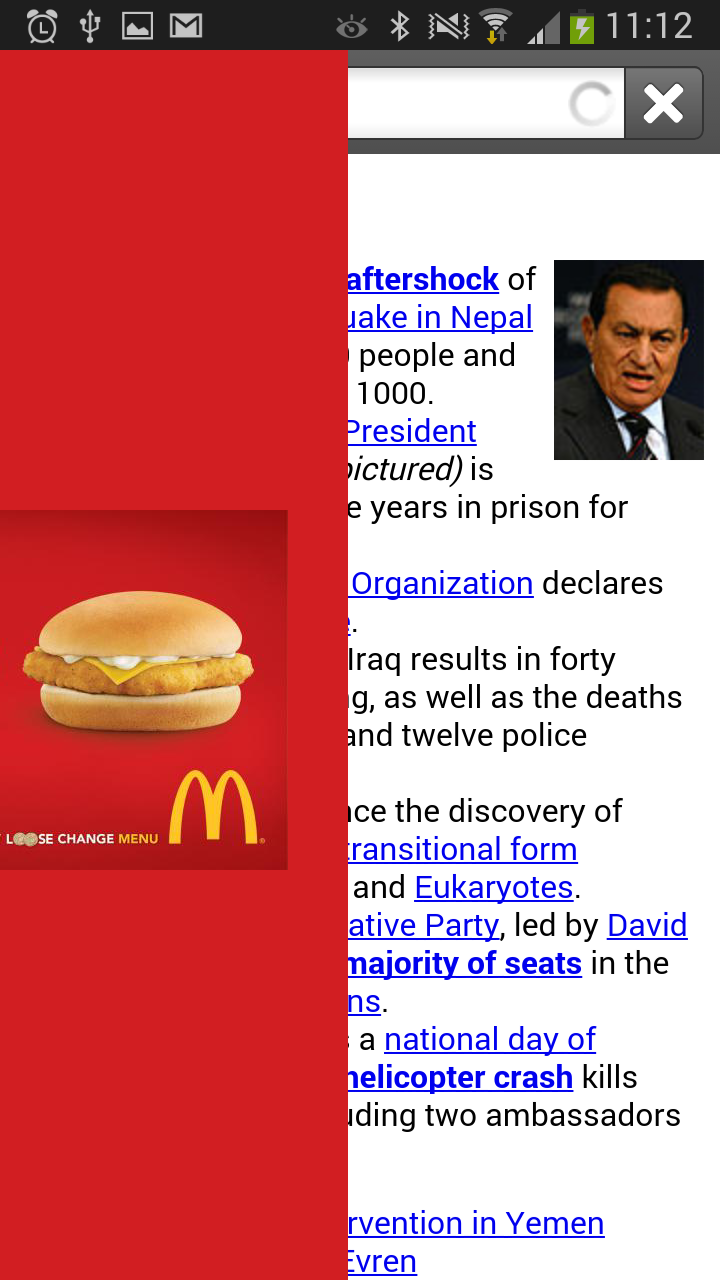
\includegraphics[scale=0.25]{Images/gesturead_big2.png}
\caption{Examples of the application with a \textit{Gestrure Ad} in maximised form displayed}
\label{fig:ads3}
\end{center}
\end{figure}

To measure how users view the proposed method, a questionnaire was composed. [Appendix A] It consists of 14 questions. 10 of the questions are about day-to-day application usage and opinion on traditional mobile advertisements. The final four questions are pertaining to the dynamic nature of the advertisement and how it compares to advertisements the participants are used to seeing in applications.

There were 25 participants between the ages of 20 and 35, all day-to-day smartphone users. 64\% of the participants were male.

They were asked to answer the first ten questions. Then they were asked to read an article of their choice from the Wikipedia application, half way though which an advertisement appeared, and asked to answer the final four questions.

\section{Results}

\subsection{Participants' Opinion on Traditional Mobile Advertising}

The participants claimed to be using their mobile devices anywhere between less than 30 minutes and more than 3 hours, however more than half of the participants use their mobile device 30 minutes to 1 hour each day as seen on Figure \ref{q1}.

\begin{figure}
\begin{center}
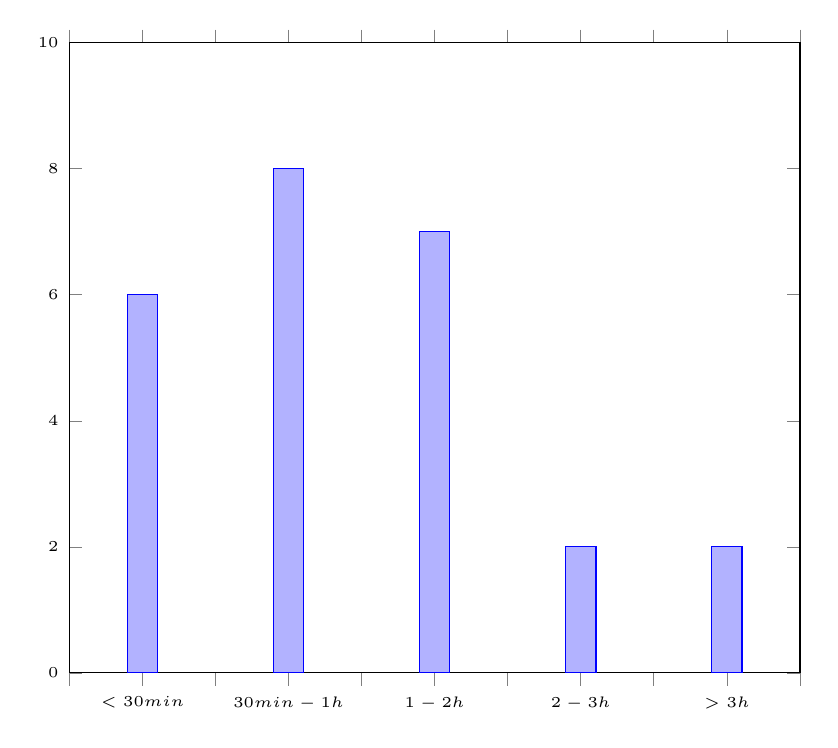
\begin{tikzpicture}[scale=1.1]

\begin{axis}[
style={font=\tiny},
ybar,
scale only axis,
xmin=0, xmax=20,
xticklabels={, ,$<30min$, ,$30min-1h$, ,$1-2h$, ,$2-3h$, ,$>3h$},
ymin=0, ymax=10,
]

\addplot coordinates{ (2,6) (6,8) (10,7) (14,2) (18,2)};

\end{axis}
\end{tikzpicture}
\caption{Participants' mobile device usage}
\label{q1}
\end{center}
\end{figure}

The average rating the participants gave to classical mobile advertisements bothering them is 3.72 on a scale from 1 to 5, 1 meaning not at all and 5 meaning very much. None of the participants claimed that mobile advertisements did not bother them at all as seen on Figure \ref{q2}. Many reasons were pointed out why advertisements are bothersome. The main ones being that the advertisements are distracting from using the application (flashing, sounds), take up a lot of screen space and are sometimes difficult or even impossible to get rid of.

\begin{figure}
\begin{center}
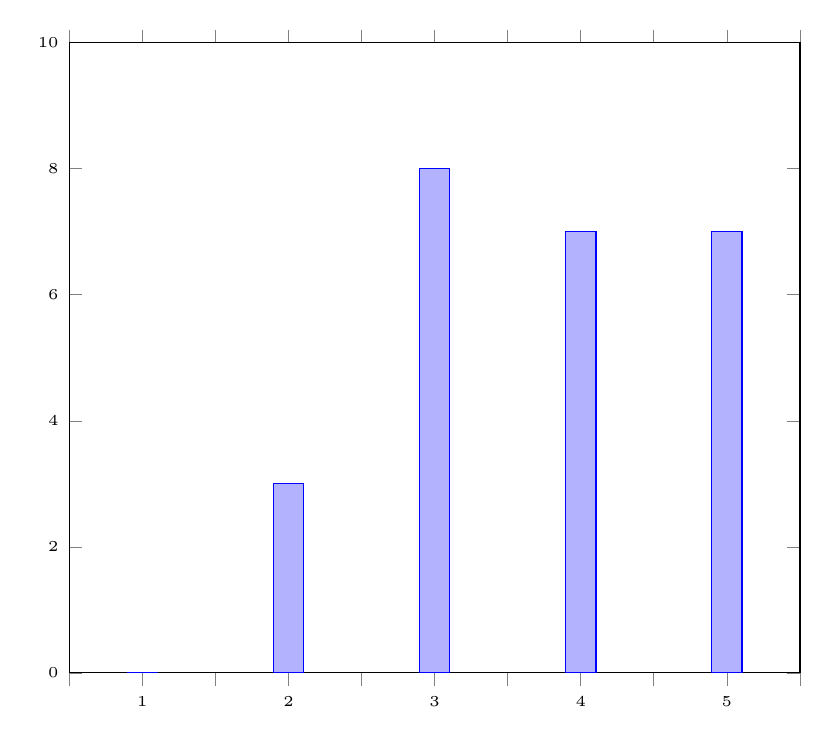
\begin{tikzpicture}[scale=1.1]

\begin{axis}[
style={font=\tiny},
ybar,
scale only axis,
xmin=0, xmax=20,
xticklabels={, ,$1$, ,$2$, ,$3$, ,$4$, ,$5$},
ymin=0, ymax=10,
]

\addplot coordinates{ (2,0) (6,3) (10,8) (14,7) (18,7)};

\end{axis}
\end{tikzpicture}
\caption{How much participants are bothered by advertisements in mobile applications}
\label{q2}
\end{center}
\end{figure}

Furthermore, 84\% of the participants claim to have uninstalled a mobile application just because of the intrusiveness of it's advertisements as seen on Figure \ref{q3}, while only 28\% claim to have looked up a product or service because of an advertisement in an application as seen on Figure \ref{q4} and only 8\% to have actually paid for a product or service they saw in an advertisement as seen on Figure \ref{q5}.

\begin{figure}
\begin{center}
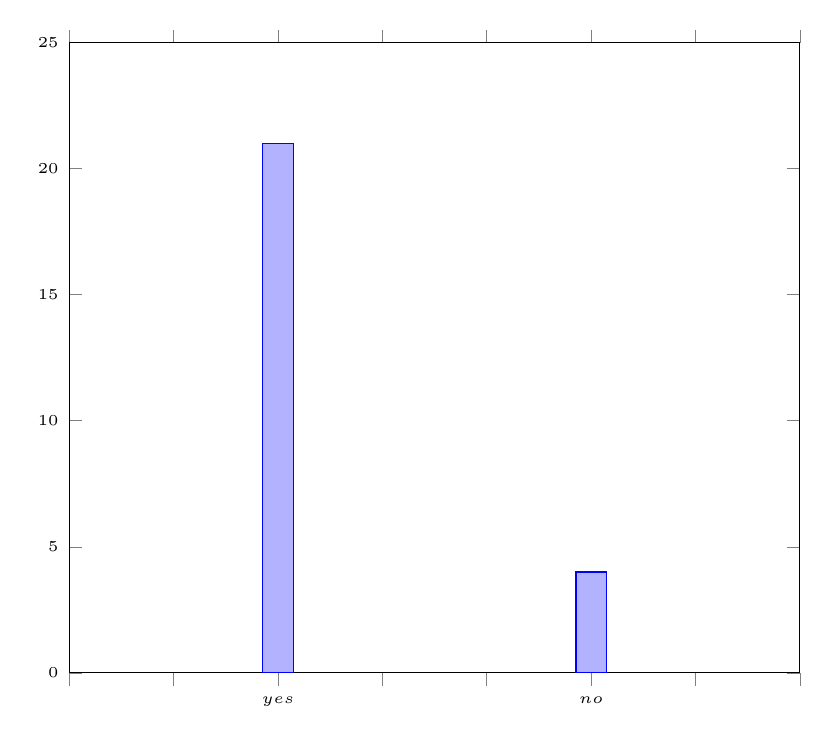
\begin{tikzpicture}[scale=1.1]

\begin{axis}[
style={font=\tiny},
ybar,
scale only axis,
xmin=0, xmax=3.5,
xticklabels={, , ,$yes$, , ,$no$},
ymin=0, ymax=25,
]

\addplot coordinates{ (1,21) (2.5,4) };

\end{axis}
\end{tikzpicture}
\caption{How many participants have uninstalled an application because of intrusive advertisements}
\label{q3}
\end{center}
\end{figure}

\begin{figure}
\begin{center}
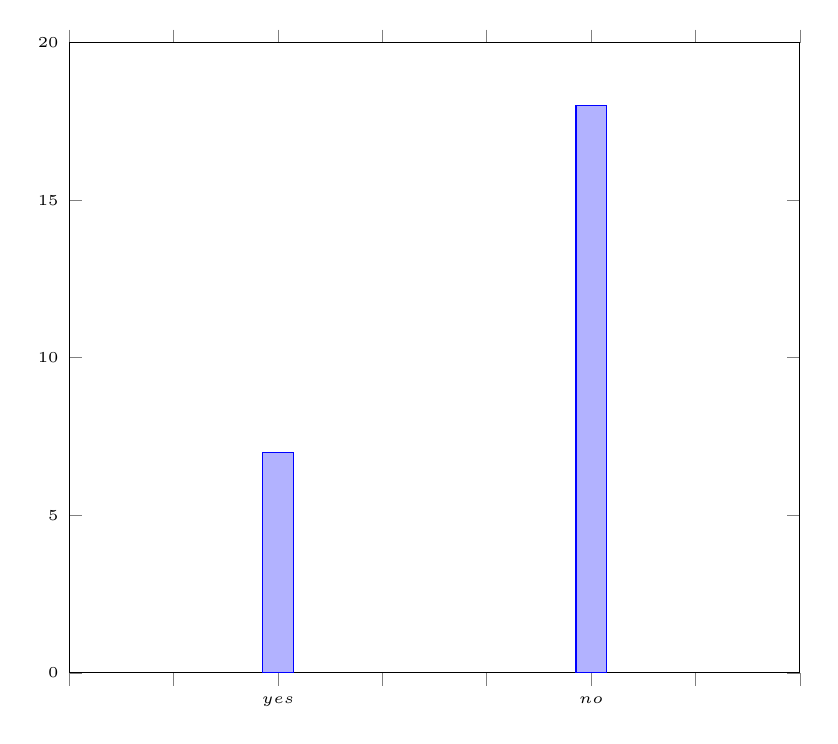
\begin{tikzpicture}[scale=1.1]

\begin{axis}[
style={font=\tiny},
ybar,
scale only axis,
xmin=0, xmax=3.5,
xticklabels={, , ,$yes$, , ,$no$},
ymin=0, ymax=20,
]

\addplot coordinates{ (1,7) (2.5,18) };

\end{axis}
\end{tikzpicture}
\caption{How many participants have looked up a product or a service because of a mobile advertisement}
\label{q4}
\end{center}
\end{figure}

\begin{figure}
\begin{center}
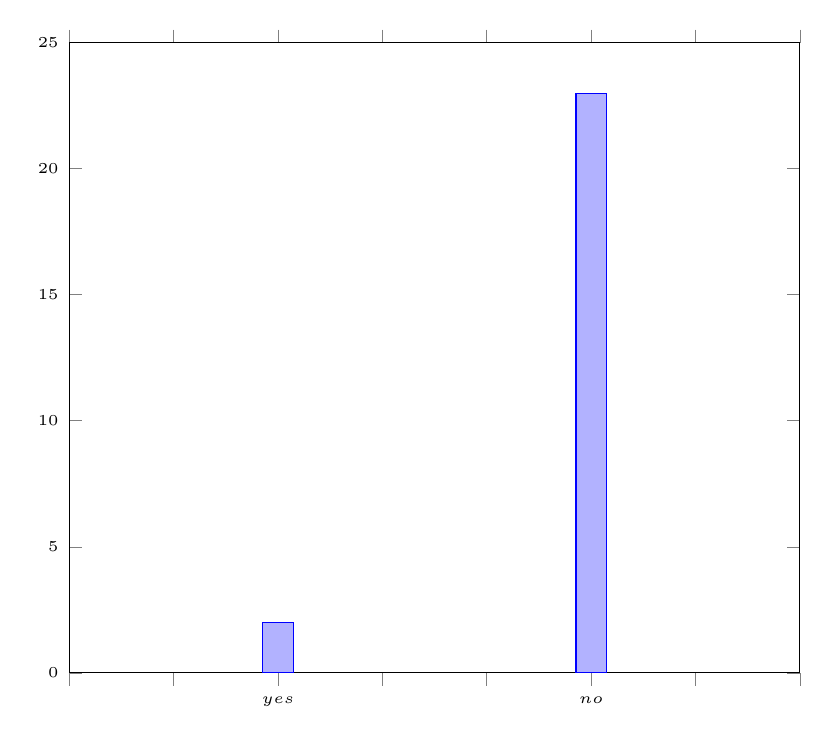
\begin{tikzpicture}[scale=1.1]

\begin{axis}[
style={font=\tiny},
ybar,
scale only axis,
xmin=0, xmax=3.5,
xticklabels={, , ,$yes$, , ,$no$},
ymin=0, ymax=25,
]

\addplot coordinates{ (1,2) (2.5,23) };

\end{axis}
\end{tikzpicture}
\caption{How many participants have paid for a product or a service because of a mobile advertisement}
\label{q5}
\end{center}
\end{figure}

This shows how ineffective traditional advertising methods are and that people are quite easily willing to stop using an application that has intrusive adverts. Traditional advertising methods are often quantity-over-quality and developers can easily damage their reputation without significant gain.

\subsection{Participants' Willingness to Adapt to New Methods of Advertising}

The participants were asked questions about their willingness to use functionality that this library provides without having used it before, to see whether they would be willing to adapt to dynamic advertisements in the applications they use\footnote{http://}.

All the participants thought they would get rid of an advertisement as soon as it appeared at least half the time as seen on Figure \ref{q6}, but 44\% of participants thought they would move an advertisement for later viewing at least some of the times and 24\% that they would want to view an advertisement later about half the times as seen on Figure \ref{q7}.

\begin{figure}
\begin{center}
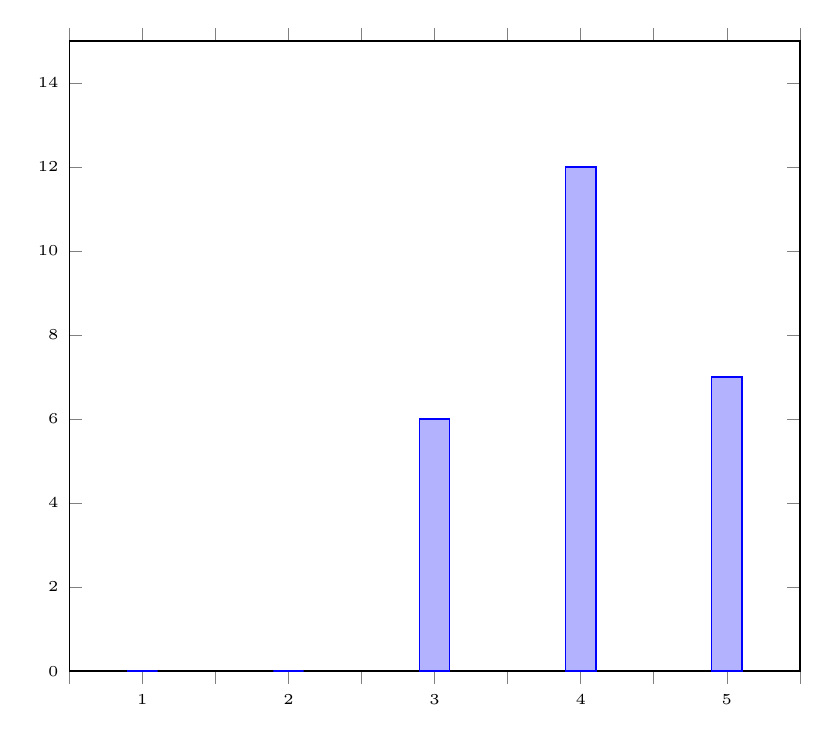
\begin{tikzpicture}[scale=1.1]

\begin{axis}[
style={font=\tiny},
ybar,
scale only axis,
xmin=0, xmax=20,
xticklabels={, ,$1$, ,$2$, ,$3$, ,$4$, ,$5$},
ymin=0, ymax=15,
]

\addplot coordinates{ (2,0) (6,0) (10,6) (14,12) (18,7)};

\end{axis}
\end{tikzpicture}
\caption{How likely participants would move an advertisement for later viewing}
\label{q6}
\end{center}
\end{figure}

\begin{figure}
\begin{center}
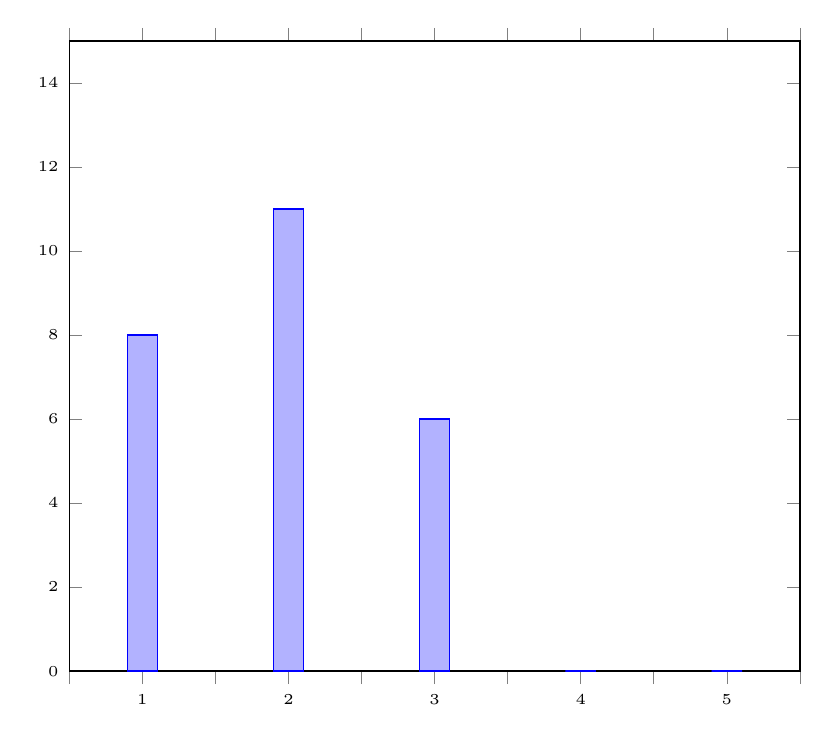
\begin{tikzpicture}[scale=1.1]

\begin{axis}[
style={font=\tiny},
ybar,
scale only axis,
xmin=0, xmax=20,
xticklabels={, ,$1$, ,$2$, ,$3$, ,$4$, ,$5$},
ymin=0, ymax=15,
]

\addplot coordinates{ (2,8) (6,11) (10,6) (14,0) (18,0)};

\end{axis}
\end{tikzpicture}
\caption{How likely participants would get rid of an advertisement as soon as it appeared}
\label{q7}
\end{center}
\end{figure}

When asked how they themselves think advertisements should be displayed in applications to make them less disruptive, the most common answers were that the advertisements should be smaller, blend in with the surroundings more and not be on top of content.

As seen from this feedback, the users would, at least some of the time, be willing to use the functionality this library provides for advertisements. Also, it has many of the features the users themselves proposed for making adverts more user friendly, like being smaller and not being on top of content the users wishes to interact with.

\section{Participants' Opinion of Dynamic Advertisements}

In terms of intrusiveness, all participants thought that the proposed method is less or just as intrusive as the classical method of advertisement delivery. 24\% thought that it is considerably less intrusive and 36\% that is just as intrusive as seen on Figure \ref{q8}.

\begin{figure}
\begin{center}
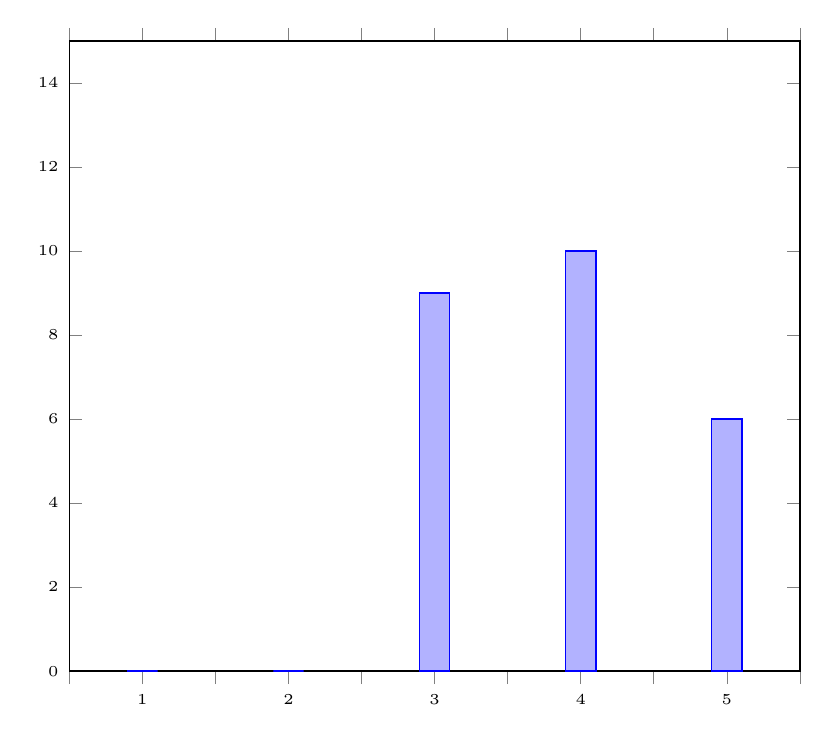
\begin{tikzpicture}[scale=1.1]

\begin{axis}[
style={font=\tiny},
ybar,
scale only axis,
xmin=0, xmax=20,
xticklabels={, ,$1$, ,$2$, ,$3$, ,$4$, ,$5$},
ymin=0, ymax=15,
]

\addplot coordinates{ (2,0) (6,0) (10,9) (14,10) (18,6)};

\end{axis}
\end{tikzpicture}
\caption{Intrusiveness comparison}
\label{q8}
\end{center}
\end{figure}

48\% of participants were just as interested in the advertised product as they would have been with the classical advertising method. 40\% were a little bit more interested and the product. 12\% were considerably more interested as seen on Figure \ref{q9}.

\begin{figure}
\begin{center}
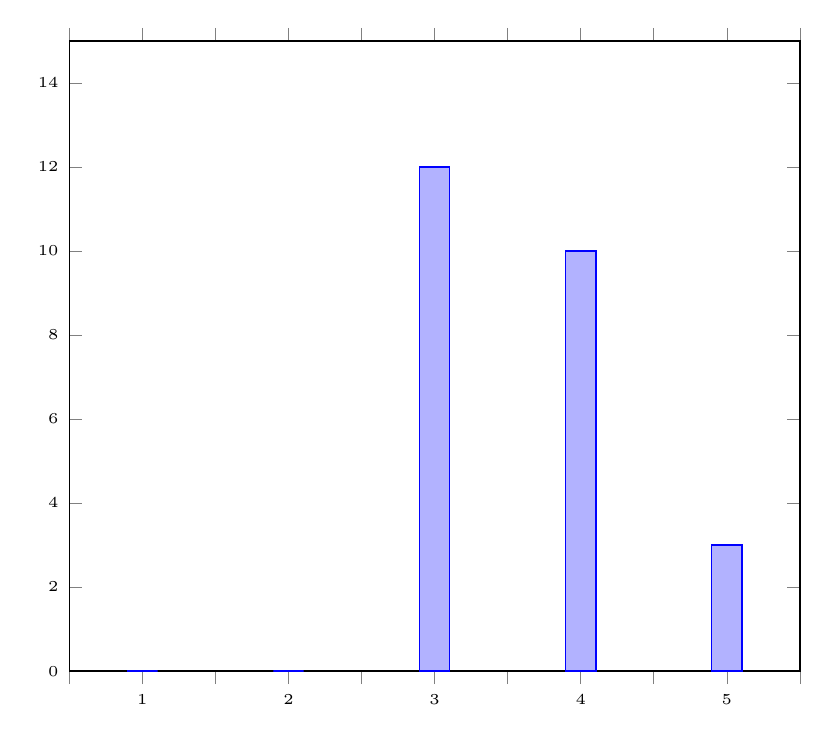
\begin{tikzpicture}[scale=1.1]

\begin{axis}[
style={font=\tiny},
ybar,
scale only axis,
xmin=0, xmax=20,
xticklabels={, ,$1$, ,$2$, ,$3$, ,$4$, ,$5$},
ymin=0, ymax=15,
]

\addplot coordinates{ (2,0) (6,0) (10,12) (14,10) (18,3)};

\end{axis}
\end{tikzpicture}
\caption{Interest comparison}
\label{q9}
\end{center}
\end{figure}

The general rating participants gave to the method of advertisement delivery is 3.96 on a scale from 1 to 5 as seen on Figure \ref{q10}.

\begin{figure}
\begin{center}
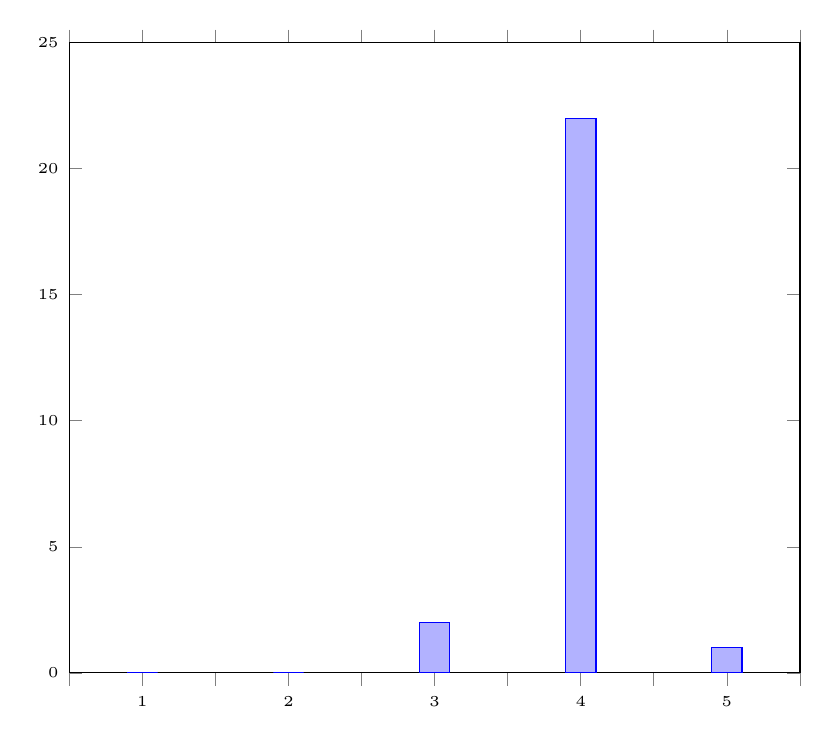
\begin{tikzpicture}[scale=1.1]

\begin{axis}[
style={font=\tiny},
ybar,
scale only axis,
xmin=0, xmax=20,
xticklabels={, ,$1$, ,$2$, ,$3$, ,$4$, ,$5$},
ymin=0, ymax=25,
]

\addplot coordinates{ (2,0) (6,0) (10,2) (14,22) (18,1)};

\end{axis}
\end{tikzpicture}
\caption{Rating}
\label{q10}
\end{center}
\end{figure}

\section{Summary}

In this chapter the usage of the proposed mechanism is validated. Based on the results, 64\% of the participants found the mechanism to be less intrusive than classical advertising. 52\% of the participants reported being more interested in the advertised product.

Almost all users found that being able to move an advertisement around on the screen is something that they would like to do in mobile applications. Some found that, being used to classical advertisements, the fact that the advertisement can be interacted with is not very intuitive and needs instructions on first application launch.

Some of the participants are application developers and were more than happy to start using this method for application monetization if it ever became a feasible option.							% functional scenario
\chapter{Conclusions and Future Directions}

Sending personalised advertisements to a user's smartphone is one the most intimate advertising channels. The excessive use of it, however, has become a serious problem. Excessive amount of advertisements in mobile applications degrade the user experience and make the user view the advertisements in a negative light. The effectiveness of such advertising questionable as well.

To mitigate this problem, a library was developed that presents advertisements in mobile applications in a more user friendly manner. It lets the user move it around on the screen according to need or move it off the screen altogether. If the user chooses to keep it on the screen for later viewing, the advertisement is small enough that it does not distract from using the application. In addition, users themselves can give feedback on the advertisements, which more accurately helps send more relevant advertisements in the future, instead of relying on profiling algorithms to decide the user's likes and dislikes.

However, the developed solution is just a proof of concept and has far a way to go for being usable in an actual real world solution. The client side of the library needs stability improvements and rigorous testing. The animations could be improved and the user interface made more intuitive to use.

The server-side needs to be built from scratch, with improvements in security and stability. Also, keeping in mind that an advertising framework needs to handle a large amount of users at any given time, which the current solution can not.

In the future, this mechanism will be merged with a mood tracking framework present advertisements to the user based on emotions. This coupled with feedback that the user provides, should very accurately describe the user's interests at any given time.

All in all, the feedback received from the control group was mainly positive. This gives hope that, in the future, a state can be reached, where mobile advertisements are construed as a useful and positive thing by an application user, rather than an annoyance and encourages exploring new directions in mobile advertising.							% final conclusions
%\include{6/relatedwork}	                	% related work
%
% this file is called up by thesis.tex
% content in this file will be fed into the main document

\chapter{Future Research Directions} % top level followed by section, subsection

% ----------------------- paths to graphics ------------------------

% change according to folder and file names
\ifpdf
    \graphicspath{{8/figures/PNG/}{8/figures/PDF/}{8/figures/}}
\else
    \graphicspath{{8/figures/EPS/}{8/figures/}}
\fi

% ----------------------- contents from here ------------------------

% ---------------------------------------------------------------------------
%: ----------------------- end of thesis sub-document ------------------------
% ---------------------------------------------------------------------------					% future research directions
%\begin{abstracts}

\textbf{D\"{u}naamilised Reklaamid Mobiilirakendustele}

T\"{a}nap\"{a}eval on reklaamid lahutamatu osa mobiilirakenduste arendusest. Paljudel juhtudel lasevad reklaamid arendajal oma rakendust kasutajatele tasuta pakkuda. Siiski, reklaamid mobiilirakendustes segavad sageli kasutajat ning sageli muudavad rakenduse kasutamise nii ebamugavaks, et kasutaja otsustab rakenduse kasutamise sootuks l\~{o}petada. Lisaks baseerub reklaamide sisu ebausaldusv\"{a}\"{a}rsete algoritmide tulemustel ning ei pruugi kajastada kasutaja tegelikke huve.

V\"{a}ljapakutud lahendus sellele probleemile on n\"{a}idata rekandusesisest reklaami kasutajale d\"{u}naamilisemal kujul; sellisel moel, et reklaam tunduks nagu osa rakendusest, mitte selle ebameeldiv lisa; ning lasta kasutajatel endil anda tagasisidet selle kohta, millised reklaamid neile huvi pakuvad ning millised mitte.

H\"{u}poteesi kontrollimiseks arendatakse selline mehhanism Androidi teegi, ning kaasask\"{a}iva serverirakenduse, kujul. Kasutusloona lisatakse see \"{u}hele mobiilirakendusele, et demonstreerida sellise l\"{a}henemise kasulikkust.

64\% rakendust proovinud kasutajatest arvas, et see mehhanism on v\"{a}hem h\"{a}iriv kui klassikalised meetodid reklaami n\"{a}itamiseks. 52\% kasutajatest v\"{a}itis end olevat reklaami sisust rohkem huvitatud.

Need tulemust n\"{a}itavad, kui ebaefektiivsed on klassikalised reklaamid mobiili-rakendustes ning julgustavad uurima uusi suundi mobiilse reklaami n\"{a}itamiseks.

\bigskip

\textbf{V\~{o}tmes\~{o}nad:} Mobiilne, Android, Reklaam, K\"{a}eliigutused

\end{abstracts}               		% discussion of results

% --------------------------------------------------------------
%:                  BACK MATTER: appendices, refs,..
% --------------------------------------------------------------

% the back matter: appendix and references close the thesis

%: ----------------------- appendices ------------------------

\chapter{Appendices}

\appendix{
\section*{Appendix A}
%: ----------------------- contents from here ------------------------

\begin{enumerate}
  \item How much do you use applications on a mobile device on an average day?
  
1	\tab\tab	2	\tab\tab	3	\tab\tab	4	\tab\tab	5
  		
  \item Rate how much advertisements bother you when using mobile applications, where 5 is very much and 1 is not at all.
  
1	\tab\tab	2	\tab\tab	3	\tab\tab	4	\tab\tab	5  
  
  \item If you chose more than 1, explain quickly what bothers you most about mobile advertising?
  
\noindent\makebox[\linewidth]{\rule{\textwidth}{0.4pt}}
\noindent\makebox[\linewidth]{\rule{\textwidth}{0.4pt}}
\noindent\makebox[\linewidth]{\rule{\textwidth}{0.4pt}}
  
  \item Have you even uninstalled and application just because of the intrusiveness of advertisements?
  
YES	\tab\tab	NO
  
  \item Have you ever looked up a product or service because you saw an advertisement of it in a mobile application?
  
YES	\tab\tab	NO  
  
  \item Have you ever bought a product or payed for a service because you saw an advertisement of it in a mobile application?
  
YES	\tab\tab	NO  
  
  \item Given the chance, how often would you get rid of an advertisement as soon as it appeared on the screen, without paying any attention to its content, where 5 is always and 1 is never?
  
1	\tab\tab	2	\tab\tab	3	\tab\tab	4	\tab\tab	5  
  
  \item Given the chance, how often would you move an advertisement to a different location for later viewing, where 5 is always and 1 is never?
  
1	\tab\tab	2	\tab\tab	3	\tab\tab	4	\tab\tab	5  
  
  \item Given the chance, how often would you give honest feedback on whether you like an advertisement or not to, in the future, get advertisements based on your interests, where 5 is always and 1 is never?
  
1	\tab\tab	2	\tab\tab	3	\tab\tab	4	\tab\tab	5  
  
  \item How would you like advertisements in your mobile applications to be displayed to make their presence less disruptive?
  
\noindent\makebox[\linewidth]{\rule{\textwidth}{0.4pt}}
\noindent\makebox[\linewidth]{\rule{\textwidth}{0.4pt}}
\noindent\makebox[\linewidth]{\rule{\textwidth}{0.4pt}}
  
  \item Rate how you would compare this method of advertisement delivery to the classical one you see in mobile applications usually (banners, full-screen interstitials) in terms of intrusiveness, where 5 is considerably less intrusive and 1 is considerably more intrusive.
  
1	\tab\tab	2	\tab\tab	3	\tab\tab	4	\tab\tab	5  
  
  \item Rate how you would compare this method of advertisement delivery to the classical one you see in mobile applications usually (banners, full-screen interstitials) in terms of your interest in the advertised product, where 5 is considerably more interested and 1 is considerably less interested.
  
1	\tab\tab	2	\tab\tab	3	\tab\tab	4	\tab\tab	5  
  
  \item Give your general opinion about this method in a few sentences.
  
\noindent\makebox[\linewidth]{\rule{\textwidth}{0.4pt}}
\noindent\makebox[\linewidth]{\rule{\textwidth}{0.4pt}}
\noindent\makebox[\linewidth]{\rule{\textwidth}{0.4pt}}
  
  \item Give a general rating about this method, where 5 is best and 1 is worst.
  
1	\tab\tab	2	\tab\tab	3	\tab\tab	4	\tab\tab	5  
  
\end{enumerate}

% ---------------------------------------------------------------------------
%: ----------------------- end of thesis sub-document ------------------------
% ---------------------------------------------------------------------------
}

\appendix{
\section*{Appendix B}
\section*{\small Non-exclusive licence to reproduce thesis and make thesis public}


I, \textbf{Jaan Tohver} (date of birth: 14th of June 1991),

\begin{tabbing}
\= Xiii\=\kill
\>1. \> herewith grant the University of Tartu a free permit (non-exclusive licence) to:\\\\ 

\>1.1\> 
\begin{minipage}[t]{14.2cm}
reproduce, for the purpose of preservation and making available to the public, including for addition to the DSpace digital archives until expiry of the term of validity of the copyright, and
\end{minipage}
\\\\
\>1.2 
\begin{minipage}[t]{14.2cm}
make available to the public via the web environment of the University of Tartu, including via the DSpace digital archives until expiry of the term of validity of the copyright,\\ 

Gesture Ads for Smartphone Applications\\   

supervised by Huber Flores, MSc and Satish Srirama, PhD

\end{minipage}\\\\ 
\>2. \>I am aware of the fact that the author retains these rights.\\\\
\>3. \>
\begin{minipage}[t]{14.2cm}
I certify that granting the non-exclusive licence does not infringe the intellectual property rights or rights arising from the Personal Data Protection Act. 
\end{minipage}\\
\end{tabbing}

\noindent
Tartu, 14.05.2015
}

%: ----------------------- bibliography ------------------------

% The section below defines how references are listed and formatted
% The default below is 2 columns, small font, complete author names.
% Entries are also linked back to the page number in the text and to external URL if provided in the BibTex file.

% PhDbiblio-url2 = names small caps, title bold & hyperlinked, link to page 
\begin{multicols}{2} % \begin{multicols}{ # columns}[ header text][ space]
\begin{tiny} % tiny(5) < scriptsize(7) < footnotesize(8) < small (9)

%\bibliographystyle{Latex/Classes/PhDbiblio-url2} % Title is link if provided
%\renewcommand{\bibname}{References} % changes the header; default: Bibliography

%\bibliography{9_backmatter/references} % adjust this to fit your BibTex file


\bibliographystyle{elsarticle-num}	% references style
\bibliography{thesis}						% references bibtex file  - utilize JabRef

\end{tiny}
\end{multicols}

% --------------------------------------------------------------
% Various bibliography styles exit. Replace above style as desired.

% in-text refs: (1) (1; 2)
% ref list: alphabetical; author(s) in small caps; initials last name; page(s)
%\bibliographystyle{Latex/Classes/PhDbiblio-case} % title forced lower case
%\bibliographystyle{Latex/Classes/PhDbiblio-bold} % title as in bibtex but bold
%\bibliographystyle{Latex/Classes/PhDbiblio-url} % bold + www link if provided

%\bibliographystyle{Latex/Classes/jmb} % calls style file jmb.bst
% in-text refs: author (year) without brackets
% ref list: alphabetical; author(s) in normal font; last name, initials; page(s)

%\bibliographystyle{plainnat} % calls style file plainnat.bst
% in-text refs: author (year) without brackets
% (this works with package natbib)


% --------------------------------------------------------------

\end{document}